\section{Discovery of Neutral Currents \cite{NC}}
The neutral currents were discovered with a neutrino beam at the bubble chamber Gargamelle. It was the first experimental proof of the theory for the electroweak unification and lead to the acceptance to describe the standard model with quantum field theories.
\subsection{Theoretical principles}
Till the begining of the 1930 the $\beta$ decay $n\rightarrow p + e^{-}$ was under as a two body decay. In this case angular momentum conservation is violated and it was not possible to explain the experimentally observed continuously energy spectrum of the electron. The solution to this problem was given by W. Pauli in 1930. He postulated a at the time unkown, uncharged and extremly light particle with a half numbered spin. This particle is today known as a neutrino and concludes the $\beta$ decay. In 1933 introduced E. Fermi the classical theory of the weak interaction. It was described by a point interaction of four fermions. The theory is just valid for the low energy limes, since it is not renormalizable.\\
The V-A structure of the weak interaction was first proposed in 1948 by Feynman and Gell-Mann as well as Marshal and Sudarshan. After the parity violation was shown by the Wu experiment, more investigations took place to understand the nature of the weak interaction. In 1968 the so called Glashow-Salam-Weinberg (GSW) model was proposed, which described the electroweak unification $SU(2)_{L}\times U(1)_{Y}$. Since the weak interaction, with the $W_{\pm}$, violates the parity conservation but the electromagnetic interaction conservers it a forth boson was needed. The Higgs mechanism broke the electroweak symmetry, as a result one of the weak and the hypercharge bosons mix to the two physical bosons $Z^0$ and $\gamma$. In addition the $W^{\pm}$ and the $Z^0$ boson get mass induced, while the photon $\gamma$ remains massless.\\
The prediction of the $Z$ boson immediately leads to the existence of neutral currents. The in 1963 introduced Cabibbo angle explained the difference between weak eigenstates and mass eigenstates. This theory allowed flavour changing neutral currents (FCNC), but experimental results showed that they are strongly suppressed. The solution was given by the GIM mechanism in 1970. The proposal of an additional charm $c$ quark lead to the result that FCNC are suppressed due to the $Z^0$ boson.\\
The search for neutral currents was not a priority of the experiments by the time. This changed in 1971 as G. `t Hooft proved that the GSW model is renormalizable.
\subsection{Experimental setup}
The Gargamelle experiment was the biggest one at the time. The advantage of this is that the long pathlength of entering particles make it possible to distingluish muons and pions and study the hadronic decay of the neutron. The exponentiel absorption of the neutrons fits completely into the chamber, which gives the possibility to study the course as well as the angular distribution. This was later very imporant to study the neutron background of the neutral current events.
The basic principle of a bubble chamber is that a liquid enters a metastable phase by heating it below its boiling point and decreasing the preasure afterwards. If a charged particle now hits the chamber it leaves a ionisation track which leads to bubbles that can be photographed. Usually a magnetic field sourronds the chamber to bend the particle tracks. This allows to determine the momentum. The Gargamelle chamber had a volume of $V=\SI{12}{\meter\cubic}$ and a magnetic field of $B=\SI{2}{\tesla}$. The used liquid was Freon. To provide the neutrino beam a proton beam with a center of mass energy of $\sqrt{s} = \SI{26}{\giga\electronvolt}$ was extracted at CERNs Proton Synchrotron (PS) and adjust onto a berylium target. By this kaons and pions get produced which will be focused through a magnetic horn and afterwards decay weakly in the \SI{70}{\meter} long decay tunnel. In front of the bubble chamber is a iron shielding so just the neutrinos can enter the chamber. To determine the neutrino flux the muon flux was measured since they are propotional.
\subsection{Measurement and results}
\begin{wrapfigure}{l}{0.35\textwidth}
    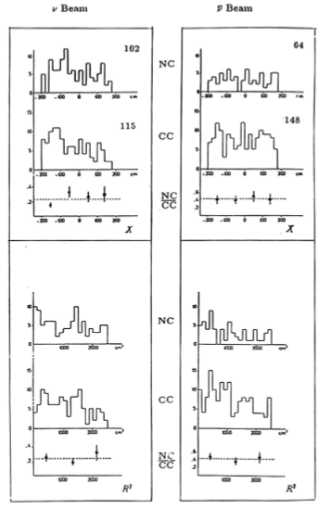
\includegraphics[width=0.33\textwidth]{graphics/CC_NC.png}
    \caption{Longitudinal and radial distribution of neurtral current and charged current events.\cite{NC}}
		\label{fig:NCCC}
  \end{wrapfigure}
  \FloatBarrier
The typical measurement of an energy distribution was not possible since it was not known how much energy the neutrino carries. It was solve my measuring the rate $R=\frac{NC}{CC}$ of the neutral currents compared to the charged current events.\\
The process associated with the charged current is $n + \nu_{\mu} \rightarrow p + \mu^{-}$ and with the neutral current $p + \nu_{\mu} \rightarrow p + \nu_{\mu}$.
Figure \ref{fig:NCCC} shows the counted events that are associated with neutral currents and charged currents. The left side shows the results for the $\nu$ beam and the right for the $\bar{\nu}$ beam. The top diagrams correspond to the longitudinal and the bottom ones to the radial position. For both confirgurations the ratio is significant different from zero. The next step was to study the background in detail. It is mainly evoked to neutrons entering the chamber, that a the result of hadronic cascades in the shielding. Figure \ref{fig:NCCCAS} shows possible tracks of neutral current (NC), charged current (CC) and the associated (AS) neutron events.\\
As mentioned before the bubble chamber is long enough to study several properties of the neutrons, this allows to predict the energy distributions of the neutral current events and the associated neutron events. The peaks of the distributions are at different points, so the energy cutoff of $E>\SI{1}{\giga\electronvolt}$ reduces the neutron background a little bit. But in general there are two different types of neutron events. The AS events are neutrons produced inside of the chamber, but there are also background (B) events that contain neutrons produced in the shielding \cite{NC_J}. Together they form the total neutron background and can be calculated with
\begin{align*}
  N_{\text{ges}} &= B + AS & \frac{B}{AS} = \frac{1}{\left< 1- \exp\left( \frac{-L}{\lambda} \right)\right> -1}\;.
\end{align*}
$L$ is the distance to the end of the downstream and $\lambda$ is the measured, characteristic interaction length. Both quantities have been measured and the final result was that around \SI{20}{\percent} of the measured NC events where actually neutron events.
	\begin{wrapfigure}{r}{0.3\textwidth}
	    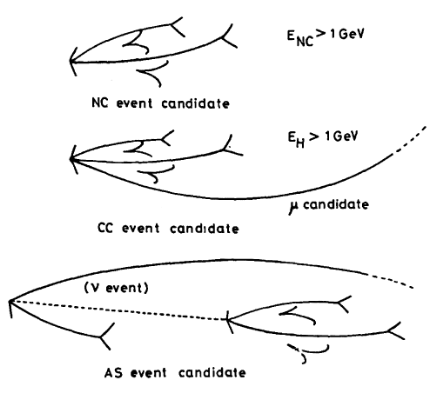
\includegraphics[width=0.28\textwidth]{graphics/CC_NC_AS.png}
	    \caption{Schematic representation of the tracks in the chamber. There are neutral current, charged current and associated events. \cite{NC_J}}
			\label{fig:NCCCAS}
	  \end{wrapfigure}
	  \FloatBarrier

Since the physics did not trust there results after a few false discoveries in the past, they applied really strict selection criteria. They include applying the high energy cut, charged events that have the possibility to not be a muon, possible cosmic events or particles that possible entered the chamber together with the beam got rejected. As well as so called $\mu$-kink events, which are muon like events with a suddenly vanishing muon track. This is a sign that it actually was a pion or proton.
The final ratio combining the results of the $\nu$ and $\bar{\nu}$ beam was
\begin{align*}
	R = 0.28 \pm 0.03
\end{align*}
This leads to the conclution that the NC events are not dominated by neutron events and neutral currents have indeed been observed. It was the first confirmation of the GSW model and lead to the nobel prize in 1979.
